\section{Ziel}
\label{sec:Ziel}
Mit diesem Experiment soll der Prozess der Phasenumwandlung von Wasser untersucht werden. Dazu wird die Dampfdruckkurve gemessen und die Verdampfungswärme $L$ bestimmt. Die Verdampfungswärme wird
dabei auf ihre Temperaturabhängigkeit untersucht.
\section{Theorie}
\label{sec:Theorie}
Damit dieses Ziel erreicht werden kann, muss zunächst verstanden werden was die Dampfdruckkurve beschreibt. Dies wird nun durch ein Beispiel mit Wasser erläutert.
Wasser nimmt mit variierender Temperatur unterschiedliche Aggregatzustände an. Ein Aggregatzustand beschreibt soetwas wie die Bewegungen der Teilchen eines Stoffen in einem bestimmten Volumen.
Die auf der Erde typischen Aggregatzustände sind fest, flüssig und gasförmig. Allerdings ist der Aggregatzustand eines Stoffes nicht nur temperaturabhängig. Der Umgebungsdruck eines Stoffes 
beeinflusst ebenfalls den Aggregatzustand. Durch diese beiden Abhängigkeiten lässt sich für einen Stoff ein Druck-Temperatur-Diagramm zeichnen. Ein solches Diagramm ist in \autoref{fig:phasenabbildung}
dargestellt.
\begin{figure}
    \centering
    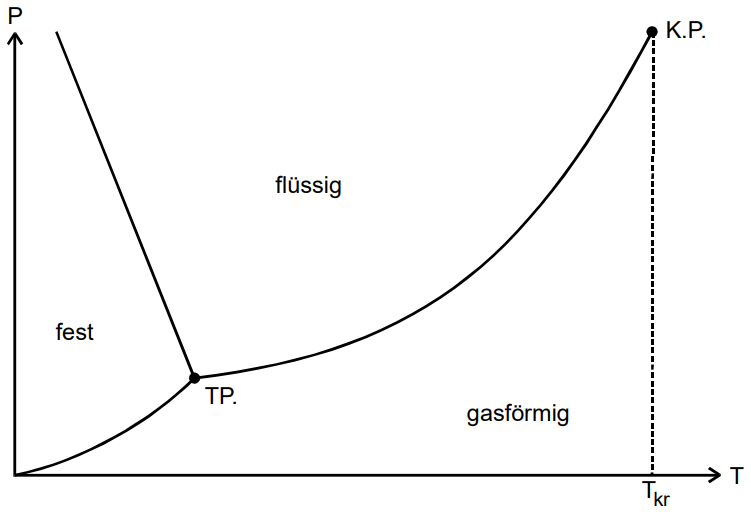
\includegraphics[width=0.8\textwidth]{content/Phasenabbildung.PNG}
	\caption{In dieser Abbildung ist der qualitative Verlauf eines Zustandsdiagramms dargestellt. \cite{v203}}
	\label{fig:phasenabbildung}
\end{figure}
Wird der Aggregatzustand von Wasser zu verschiedenen Temperaturen und Drücken untersucht, ergeben sich drei Bereiche im Diagramm, welche den drei genannten Aggregatzuständen entsprechen.  
Diese sind durch Grenzen
getrennt, wie man in \autoref{fig:phasenabbildung} erkennen kann. Die Kurve zwischen den Bereichen der Aggregatzustände flüssig und gasförmig wird Dampfdruckkurve genannt. An genau dieser Grenze besitzt das System
nur noch einen Freiheitsgrad, da bei Vorgabe eines Parameters der andere eindeutig definiert ist. Diese Kurve wird durch die zwei Punkte T.P. und K.P. begrenzt, welche in \autoref{fig:phasenabbildung}
eingezeichnet sind. Der Punkt T.P. ist der Tripelpunkt. An diesem Punkt kann Wasser alle drei Aggregatzustände annehmen, weshalb er keiner Grenzkurve eindeutig zugeordnet werden kann.
Der K.P ist ein Kritischer Punkt der Dampfdruckkurve. Ab diesem Punkt ist es auf der Dampfdruckkurve mit steigender Temperatur und steigendem Druck nicht mehr möglich zwischen den 
Aggregatzuständen "flüssig"\: und "gasförmig"\: zu unterscheiden. Daher wird die Dampfdruckkurve nur zwischen diesen beiden Punkten definiert. Eine wichtige Charakteristik der Dampfdruckkurve 
ist, dass sie im wesentlichen durch die Verdampfungswärme $L$ beschrieben werden kann. Die Verdampfungswärme ist eine wichtige Eigenschaft von Stoffen. In gewissen Temperauturbereichen kann sie
zwar als Konstante genähert werden, allerdings ist sie im Allgemeinen eine temperaturabhängige Größe. 

\subsection{Mikroskopische Vorgänge bei der Verdampfung und Kondensation}
\label{subsec:T_VK}
In diesem Versuch wird mit einer Flüssigkeit in einem evakuierten Gefäß gearbeitet. Eine Flüssigkeit in einem evakuierten Gefäß verdampft solange, bis der Druck in dem Gefäß einen Wert erreicht,
der im Zustandsdiagramm im "flüssigen"\: Bereich liegt. Bei dem eben genannten Verdampfungsprozess
geht ein Stoff vom flüssigen Zustand in den gasförmigen über. Dabei verlassen diejenigen Moleküle die Flüssigkeit, welche gemäß der Maxwellschen Geschwindigkeitsverteilung die maximale kinetische 
Energie besitzen. Bei diesem Vorgang kann sich vorgestellt werden, dass die Moleküle aufgrund ihrer Geschwindigkei aus der Flüssigkeitsoberfläche herausschießen. Damit dies geschieht, muss
ein Molekül zunächst die molekulare Bindungsenergie überwinden. Daher muss ein Molekül um zu verdampfen, entweder eine externe energetische Anregung bekommen oder die notwendige Energie
dem Wärmereservoir der Flüssigkeit entnehmen. Aufgrund dieser mikroskopischen Überlegung wird eine Größe $L_\text{mol}$ der Einheit Joule/Mol definiert, welche 
molare Verdampfungswärme genannt wird. Diese beschreibt die nötige Energie
um ein Mol einer Flüssigkeit in Dampf gleicher Temperatur umzuwandeln. Sollte ein solches Mol an Gas wieder Kondensieren, also vom gasförmigen Zustand wieder in den Flüssigen wechseln, wird genau
die Energie $L_\text{mol}$ wieder frei, beziehungsweise geht dann in das Wärmereservoir der Flüssigkeit über. Da der Druck des Gases durch Stöße mit der Umgebung verursacht wird, kann es auch passieren, dass
die Gasmoleküle mit der Flüssigkeitsoberfläche zusammenstoßen und dann wieder in die Flüssigkeit aufgenommen werden, also Kondensieren. Diese Vorgänge von Verdampfung und 
Kondensation finden kontinuierlich statt.
Nach hinreichendlanger Zeit bildet sich zwischen diesen Prozessen ein Gleichgewicht. Da der Verdampfungsprozess nicht mehr beobachtet werden kann,
wird bei diesem Gleichgewicht davon gesprochen, dass „Flüssigkeit und Dampf koexistieren". Es bildet sich ein konstanter Druck im Gas. Dieser wird Sättigungsdampfdruck genannt. Er muss mit zunehmender Temperatur ansteigen, da bei
erhöhter kinetischer Energie die Moleküle häufiger Stoßen und deshalb mehr Moleküle aus der Flüssigkeit austreten können. Der Sättigungsdampfdruck hängt nicht vom Volumen des Gefäßes ab. 
Aus diesem Grund kann das gesättigte Gas nicht durch die Allgemeine Gasgleichung beschrieben werden.
\subsection{Differentialgleichung einer Dampfdruckkurve}
\label{subsec:T_DGL}
Damit die Dampfdruckkurve nicht nur durch expermientelle Regressionen dargestellt werden kann, ist es von Interesse eine theoretische Beschreibung der Dampfdruckkurve zu finden. Dazu wird 
ein reversibler Kreisprozess von Verdampfung und Kondensation betrachtet. Dieser wird in \autoref{fig:kreisprozess} dargestellt.

\begin{figure}
    \centering
    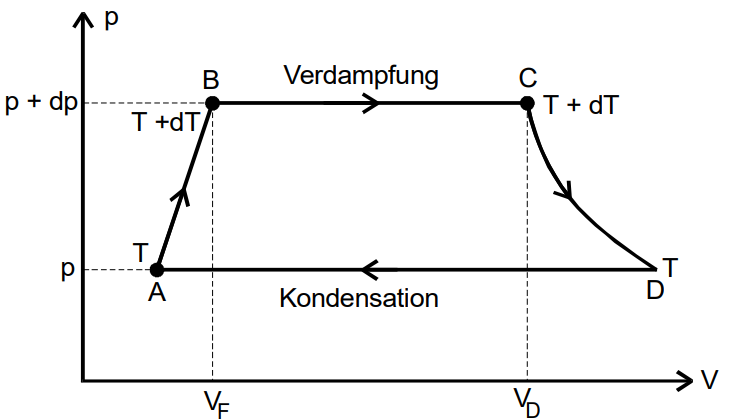
\includegraphics[width=0.8\textwidth]{content/kreisprozess.PNG}
	\caption{In dieser Abbildung ist ein Verdampfungs-Kondensations-Kreisprozess dargestellt. \cite{v203}}
	\label{fig:kreisprozess}
\end{figure}

Wie im \autoref{subsec:T_VK} beschrieben, wird bei Kondensation und Verdampfung Energie benötigt, beziehungsweise Energie abgegeben. Durch Aufstellen von Formeln für Arbeiten und Wärmemengen kann mit Hilfe
der Hauptsätze der Thermodynamik die Differentialgleichung 
\begin{equation}
    \label{eqn:DGL1}
    \left(V_\text{D} - V_\text{F}\right)\symup{d}p = \frac{L}{T}\symup{d}T
\end{equation}
aufgestellt werden, dessen Lösung die Dampfdruckkurve eines Stoffes beschreibt. $V_\text{D}$ beschreibt dabei das Volumen des Gases und $V_\text{F}$ das der Flüssigkeit.
Diese Differentialgleichung wird Clausius-Clapeyronsche Gleichung genannt.
\subsection{Integration der Clausius-Clapeyronschen Gleichung durch vereinfachende Annahmen}
\label{subsec:T_int}
Die Integration der Clausius-Clapeyronschen Gleichung ist im allgemeinen Fall schwierig, da sie durch komplizierte Temperaturabhängigkeiten ausgedrückt wird. Es werden Näherungen benötigt, welche
die Integration ermöglichen. Daher soll in guter Näherung gelten, dass $V_\text{F}$ gegenüber $V_\text{D}$ vernachlässigbar klein ist. Außerdem muss $V_\text{D}$ die ideale Gasgleichung
\begin{equation}
    \label{eqn:V_D}
    V_\text{D}(p,T) = R\frac{T}{p}
\end{equation} 
erfüllen. Die Verdampfungswärme $L$ darf dafür nicht druck- und temperaturabhängig sein. Diese Näherungen können nur als hinreichend genau betrachtet werden, solange die Temperatur
viel kleiner ist als die kritische Temperatur $T_\text{kr}$, welche in \autoref{fig:phasenabbildung} eingezeichnet ist. Sie beschreibt die obere
Temperaturgrenze der Dampfdruckkurve. Mithilfe dieser Annahmen kann nun die Differentialgleichung integriert werden. Aus \autoref{eqn:DGL1} und Annahme der \autoref{eqn:V_D} ergibt sich durch Integration
\autoref{eqn:int}.
\begin{equation}
    \label{eqn:int}
    p = p_0\text{e}^{-\frac{L}{RT}}
\end{equation}
Da \autoref{eqn:int} nur noch von den Variablen $p$ und $T$ abhängt, lässt sich diese Gleichung nach Variablen trennen. Es folgt
\begin{equation}
    \label{eqn:gerade}
    \text{ln}\left(\frac{p}{p_0}\right) = -\frac{L}{R}\frac{1}{T},
\end{equation}
woraus die Verdampfungswärme $L$ bestimmt werden kann. Aus dieser lässt sich wiederum die innere Verdampfungswärme
\begin{equation}
    \label{eqn:LI}
    L_\text{i} = L - L_\text{a}
\end{equation}
bestimmen, wobei $L_\text{a}$ die äußere Verdampfungswärme beschreibt.
